% Created by tikzDevice version 0.12.3.1 on 2022-11-14 18:16:07
% !TEX encoding = UTF-8 Unicode
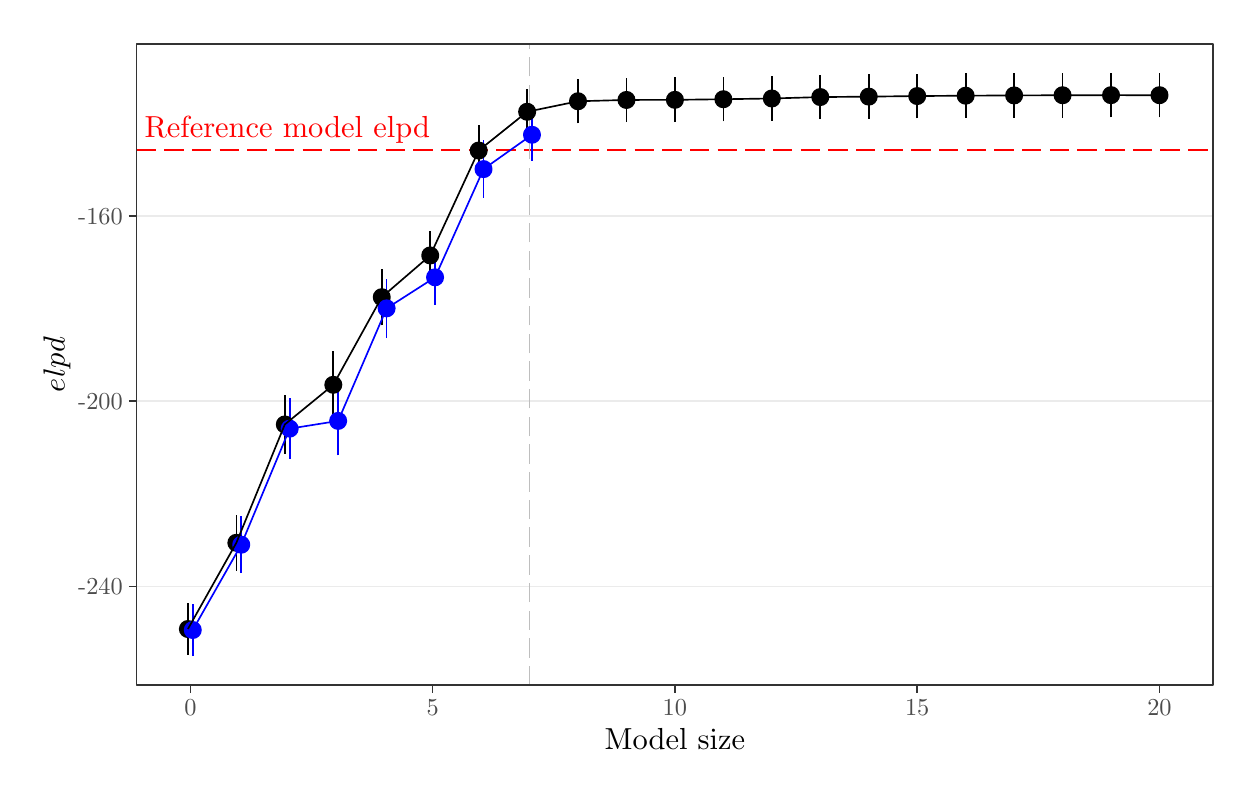
\begin{tikzpicture}[x=1pt,y=1pt]
\definecolor{fillColor}{RGB}{255,255,255}
\begin{scope}
\definecolor{drawColor}{RGB}{255,255,255}
\definecolor{fillColor}{RGB}{255,255,255}

\path[draw=drawColor,line width= 0.6pt,line join=round,line cap=round,fill=fillColor] (  0.00,  0.00) rectangle (433.62,268.00);
\end{scope}
\begin{scope}
\definecolor{fillColor}{RGB}{255,255,255}

\path[fill=fillColor] ( 39.04, 30.69) rectangle (428.12,262.50);
\definecolor{drawColor}{gray}{0.92}

\path[draw=drawColor,line width= 0.6pt,line join=round] ( 39.04, 66.34) --
	(428.12, 66.34);

\path[draw=drawColor,line width= 0.6pt,line join=round] ( 39.04,133.35) --
	(428.12,133.35);

\path[draw=drawColor,line width= 0.6pt,line join=round] ( 39.04,200.35) --
	(428.12,200.35);
\definecolor{drawColor}{RGB}{255,0,0}

\path[draw=drawColor,line width= 0.6pt,dash pattern=on 7pt off 3pt ,line join=round] ( 39.04,224.18) -- (428.12,224.18);
\definecolor{drawColor}{RGB}{190,190,190}

\path[draw=drawColor,line width= 0.6pt,dash pattern=on 7pt off 3pt ,line join=round] (181.05, 30.69) -- (181.05,262.50);
\definecolor{drawColor}{RGB}{0,0,0}

\path[draw=drawColor,line width= 0.6pt,line join=round] ( 57.60, 41.65) -- ( 57.60, 60.35);

\path[draw=drawColor,line width= 0.6pt,line join=round] ( 75.11, 72.02) -- ( 75.11, 92.31);

\path[draw=drawColor,line width= 0.6pt,line join=round] ( 92.62,114.32) -- ( 92.62,135.52);

\path[draw=drawColor,line width= 0.6pt,line join=round] (110.14,126.91) -- (110.14,151.59);

\path[draw=drawColor,line width= 0.6pt,line join=round] (127.65,160.71) -- (127.65,181.10);

\path[draw=drawColor,line width= 0.6pt,line join=round] (145.16,177.33) -- (145.16,194.65);

\path[draw=drawColor,line width= 0.6pt,line join=round] (162.67,214.77) -- (162.67,233.02);

\path[draw=drawColor,line width= 0.6pt,line join=round] (180.18,229.79) -- (180.18,246.03);

\path[draw=drawColor,line width= 0.6pt,line join=round] (198.56,233.74) -- (198.56,249.68);

\path[draw=drawColor,line width= 0.6pt,line join=round] (216.07,234.13) -- (216.07,250.23);

\path[draw=drawColor,line width= 0.6pt,line join=round] (233.58,234.14) -- (233.58,250.31);

\path[draw=drawColor,line width= 0.6pt,line join=round] (251.09,234.44) -- (251.09,250.45);

\path[draw=drawColor,line width= 0.6pt,line join=round] (268.60,234.73) -- (268.60,250.69);

\path[draw=drawColor,line width= 0.6pt,line join=round] (286.11,235.27) -- (286.11,251.17);

\path[draw=drawColor,line width= 0.6pt,line join=round] (303.62,235.36) -- (303.62,251.39);

\path[draw=drawColor,line width= 0.6pt,line join=round] (321.13,235.55) -- (321.13,251.64);

\path[draw=drawColor,line width= 0.6pt,line join=round] (338.64,235.66) -- (338.64,251.79);

\path[draw=drawColor,line width= 0.6pt,line join=round] (356.15,235.74) -- (356.15,251.87);

\path[draw=drawColor,line width= 0.6pt,line join=round] (373.66,235.83) -- (373.66,251.93);

\path[draw=drawColor,line width= 0.6pt,line join=round] (391.17,235.86) -- (391.17,251.96);

\path[draw=drawColor,line width= 0.6pt,line join=round] (408.68,235.85) -- (408.68,251.96);
\definecolor{drawColor}{RGB}{0,0,255}

\path[draw=drawColor,line width= 0.6pt,line join=round] ( 59.36, 41.22) -- ( 59.36, 60.09);

\path[draw=drawColor,line width= 0.6pt,line join=round] ( 76.87, 71.19) -- ( 76.87, 91.75);

\path[draw=drawColor,line width= 0.6pt,line join=round] ( 94.38,112.46) -- ( 94.38,134.36);

\path[draw=drawColor,line width= 0.6pt,line join=round] (111.89,113.72) -- (111.89,138.69);

\path[draw=drawColor,line width= 0.6pt,line join=round] (129.40,156.15) -- (129.40,177.60);

\path[draw=drawColor,line width= 0.6pt,line join=round] (146.91,168.20) -- (146.91,187.98);

\path[draw=drawColor,line width= 0.6pt,line join=round] (164.42,206.83) -- (164.42,227.54);

\path[draw=drawColor,line width= 0.6pt,line join=round] (181.93,220.15) -- (181.93,239.05);
\definecolor{drawColor}{RGB}{0,0,0}
\definecolor{fillColor}{RGB}{0,0,0}

\path[draw=drawColor,line width= 0.8pt,line join=round,line cap=round,fill=fillColor] ( 57.60, 51.00) circle (  2.85);

\path[draw=drawColor,line width= 0.8pt,line join=round,line cap=round,fill=fillColor] ( 75.11, 82.16) circle (  2.85);

\path[draw=drawColor,line width= 0.8pt,line join=round,line cap=round,fill=fillColor] ( 92.62,124.92) circle (  2.85);

\path[draw=drawColor,line width= 0.8pt,line join=round,line cap=round,fill=fillColor] (110.14,139.25) circle (  2.85);

\path[draw=drawColor,line width= 0.8pt,line join=round,line cap=round,fill=fillColor] (127.65,170.91) circle (  2.85);

\path[draw=drawColor,line width= 0.8pt,line join=round,line cap=round,fill=fillColor] (145.16,185.99) circle (  2.85);

\path[draw=drawColor,line width= 0.8pt,line join=round,line cap=round,fill=fillColor] (162.67,223.89) circle (  2.85);

\path[draw=drawColor,line width= 0.8pt,line join=round,line cap=round,fill=fillColor] (180.18,237.91) circle (  2.85);

\path[draw=drawColor,line width= 0.8pt,line join=round,line cap=round,fill=fillColor] (198.56,241.71) circle (  2.85);

\path[draw=drawColor,line width= 0.8pt,line join=round,line cap=round,fill=fillColor] (216.07,242.18) circle (  2.85);

\path[draw=drawColor,line width= 0.8pt,line join=round,line cap=round,fill=fillColor] (233.58,242.22) circle (  2.85);

\path[draw=drawColor,line width= 0.8pt,line join=round,line cap=round,fill=fillColor] (251.09,242.44) circle (  2.85);

\path[draw=drawColor,line width= 0.8pt,line join=round,line cap=round,fill=fillColor] (268.60,242.71) circle (  2.85);

\path[draw=drawColor,line width= 0.8pt,line join=round,line cap=round,fill=fillColor] (286.11,243.22) circle (  2.85);

\path[draw=drawColor,line width= 0.8pt,line join=round,line cap=round,fill=fillColor] (303.62,243.38) circle (  2.85);

\path[draw=drawColor,line width= 0.8pt,line join=round,line cap=round,fill=fillColor] (321.13,243.59) circle (  2.85);

\path[draw=drawColor,line width= 0.8pt,line join=round,line cap=round,fill=fillColor] (338.64,243.72) circle (  2.85);

\path[draw=drawColor,line width= 0.8pt,line join=round,line cap=round,fill=fillColor] (356.15,243.81) circle (  2.85);

\path[draw=drawColor,line width= 0.8pt,line join=round,line cap=round,fill=fillColor] (373.66,243.88) circle (  2.85);

\path[draw=drawColor,line width= 0.8pt,line join=round,line cap=round,fill=fillColor] (391.17,243.91) circle (  2.85);

\path[draw=drawColor,line width= 0.8pt,line join=round,line cap=round,fill=fillColor] (408.68,243.90) circle (  2.85);
\definecolor{drawColor}{RGB}{0,0,255}
\definecolor{fillColor}{RGB}{0,0,255}

\path[draw=drawColor,line width= 0.8pt,line join=round,line cap=round,fill=fillColor] ( 59.36, 50.65) circle (  2.85);

\path[draw=drawColor,line width= 0.8pt,line join=round,line cap=round,fill=fillColor] ( 76.87, 81.47) circle (  2.85);

\path[draw=drawColor,line width= 0.8pt,line join=round,line cap=round,fill=fillColor] ( 94.38,123.41) circle (  2.85);

\path[draw=drawColor,line width= 0.8pt,line join=round,line cap=round,fill=fillColor] (111.89,126.20) circle (  2.85);

\path[draw=drawColor,line width= 0.8pt,line join=round,line cap=round,fill=fillColor] (129.40,166.87) circle (  2.85);

\path[draw=drawColor,line width= 0.8pt,line join=round,line cap=round,fill=fillColor] (146.91,178.09) circle (  2.85);

\path[draw=drawColor,line width= 0.8pt,line join=round,line cap=round,fill=fillColor] (164.42,217.19) circle (  2.85);

\path[draw=drawColor,line width= 0.8pt,line join=round,line cap=round,fill=fillColor] (181.93,229.60) circle (  2.85);
\definecolor{drawColor}{RGB}{0,0,0}

\path[draw=drawColor,line width= 0.6pt,line join=round] ( 57.60, 51.00) --
	( 75.11, 82.16) --
	( 92.62,124.92) --
	(110.14,139.25) --
	(127.65,170.91) --
	(145.16,185.99) --
	(162.67,223.89) --
	(180.18,237.91) --
	(198.56,241.71) --
	(216.07,242.18) --
	(233.58,242.22) --
	(251.09,242.44) --
	(268.60,242.71) --
	(286.11,243.22) --
	(303.62,243.38) --
	(321.13,243.59) --
	(338.64,243.72) --
	(356.15,243.81) --
	(373.66,243.88) --
	(391.17,243.91) --
	(408.68,243.90);
\definecolor{drawColor}{RGB}{0,0,255}

\path[draw=drawColor,line width= 0.6pt,line join=round] ( 59.36, 50.65) --
	( 76.87, 81.47) --
	( 94.38,123.41) --
	(111.89,126.20) --
	(129.40,166.87) --
	(146.91,178.09) --
	(164.42,217.19) --
	(181.93,229.60);
\definecolor{drawColor}{RGB}{255,0,0}

\node[text=drawColor,anchor=base,inner sep=0pt, outer sep=0pt, scale=  1.10] at ( 93.50,228.75) {Reference model elpd};
\definecolor{drawColor}{gray}{0.20}

\path[draw=drawColor,line width= 0.6pt,line join=round,line cap=round] ( 39.04, 30.69) rectangle (428.12,262.50);
\end{scope}
\begin{scope}
\definecolor{drawColor}{gray}{0.30}

\node[text=drawColor,anchor=base east,inner sep=0pt, outer sep=0pt, scale=  0.88] at ( 34.09, 63.31) {-240};

\node[text=drawColor,anchor=base east,inner sep=0pt, outer sep=0pt, scale=  0.88] at ( 34.09,130.32) {-200};

\node[text=drawColor,anchor=base east,inner sep=0pt, outer sep=0pt, scale=  0.88] at ( 34.09,197.32) {-160};
\end{scope}
\begin{scope}
\definecolor{drawColor}{gray}{0.20}

\path[draw=drawColor,line width= 0.6pt,line join=round] ( 36.29, 66.34) --
	( 39.04, 66.34);

\path[draw=drawColor,line width= 0.6pt,line join=round] ( 36.29,133.35) --
	( 39.04,133.35);

\path[draw=drawColor,line width= 0.6pt,line join=round] ( 36.29,200.35) --
	( 39.04,200.35);
\end{scope}
\begin{scope}
\definecolor{drawColor}{gray}{0.20}

\path[draw=drawColor,line width= 0.6pt,line join=round] ( 58.48, 27.94) --
	( 58.48, 30.69);

\path[draw=drawColor,line width= 0.6pt,line join=round] (146.03, 27.94) --
	(146.03, 30.69);

\path[draw=drawColor,line width= 0.6pt,line join=round] (233.58, 27.94) --
	(233.58, 30.69);

\path[draw=drawColor,line width= 0.6pt,line join=round] (321.13, 27.94) --
	(321.13, 30.69);

\path[draw=drawColor,line width= 0.6pt,line join=round] (408.68, 27.94) --
	(408.68, 30.69);
\end{scope}
\begin{scope}
\definecolor{drawColor}{gray}{0.30}

\node[text=drawColor,anchor=base,inner sep=0pt, outer sep=0pt, scale=  0.88] at ( 58.48, 19.68) {0};

\node[text=drawColor,anchor=base,inner sep=0pt, outer sep=0pt, scale=  0.88] at (146.03, 19.68) {5};

\node[text=drawColor,anchor=base,inner sep=0pt, outer sep=0pt, scale=  0.88] at (233.58, 19.68) {10};

\node[text=drawColor,anchor=base,inner sep=0pt, outer sep=0pt, scale=  0.88] at (321.13, 19.68) {15};

\node[text=drawColor,anchor=base,inner sep=0pt, outer sep=0pt, scale=  0.88] at (408.68, 19.68) {20};
\end{scope}
\begin{scope}
\definecolor{drawColor}{RGB}{0,0,0}

\node[text=drawColor,anchor=base,inner sep=0pt, outer sep=0pt, scale=  1.10] at (233.58,  7.64) {Model size};
\end{scope}
\begin{scope}
\definecolor{drawColor}{RGB}{0,0,0}

\node[text=drawColor,rotate= 90.00,anchor=base,inner sep=0pt, outer sep=0pt, scale=  1.10] at ( 13.08,146.59) {$elpd$};
\end{scope}
\end{tikzpicture}
